
\section{Motivations}
\label{repl:sec:motivations}

\begin{figure*}
  \centering
  \subfloat[Document Wikipedia principalement édité en fin.]
  [Document Wikipedia de très grande taille principalement édité en fin.]
  {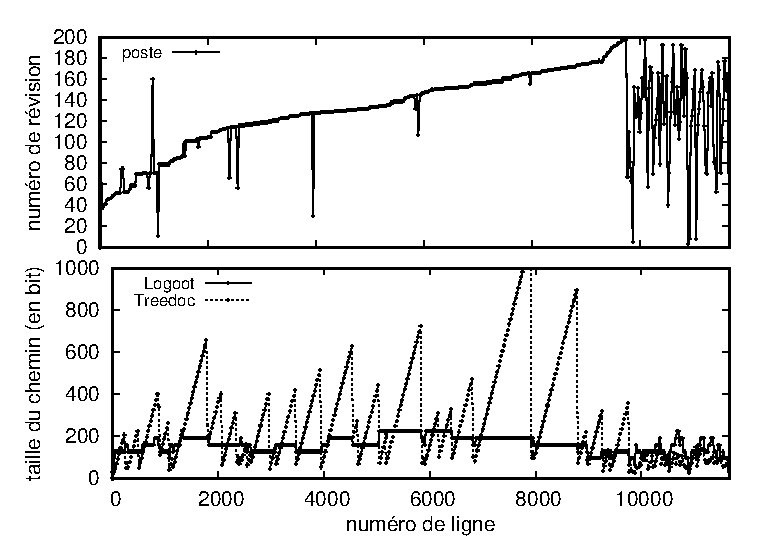
\includegraphics[width=0.48\textwidth]{img/lseq/motivationposte.eps}}
  \hspace{10pt}
  \subfloat[Document Wikipedia principalement édité au début.]
  [Document Wikipedia de petite taille principalement édité en début.]
  {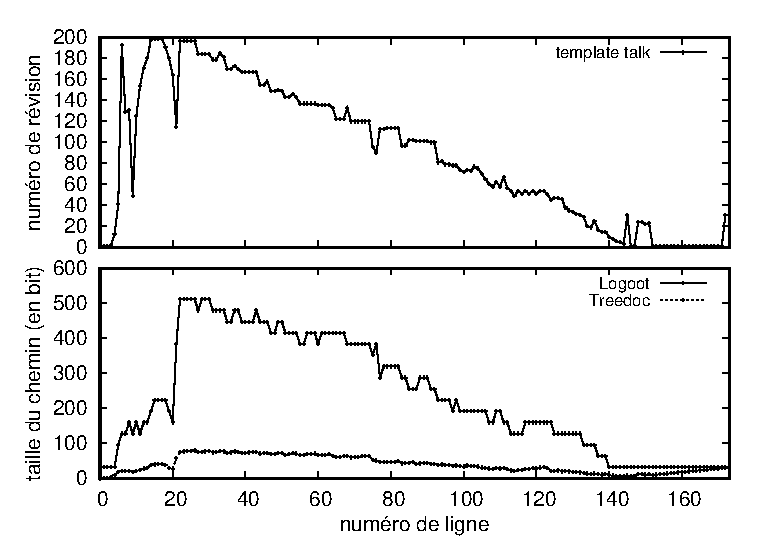
\includegraphics[width=0.48\textwidth]{img/lseq/motivationtemplatetalk.eps}}
  \caption{\label{repl:img:motivations}Motivations}
\end{figure*}



%%% Local Variables:
%%% mode: latex
%%% TeX-master: "../../paper"
%%% End:
